\documentclass[aps,prb,twocolumn,superscriptaddress,floatfix,longbibliography,nofootinbib]{revtex4-2}

\usepackage{minted, xcolor, graphicx, caption, geometry}
\usepackage{amsmath,amssymb} % math symbols
\usepackage{bm} % bold math font
\usepackage{graphicx} % for figures
\usepackage{comment} % allows block comments
%\usepackage{ulem} % allows strikeout text, e.g. \sout{text}
\usepackage[francais]{babel}

\usepackage{datetime2}
\usepackage{csquotes}
\usepackage{soul}

% Redéfinir la commande \today pour supprimer "Dated: "
% \renewcommand{\today}{\DTMdisplaydate{ \the\year}{\the\month}{\the\day}{-1}}
% \newcommand{\ajd}{\DTMdisplaydate{\the\year}{\the\month}{\the\day}{-1}}

% \usepackage[T1]{fontenc}
% \usepackage{lmodern}

\usepackage{float} % allows H in figure placement

\usepackage{minted} % allows colored code
\usepackage{textcomp} % This package gives the text quote '
\usepackage{gensymb} % This package gives the degree symbol \degree

\usepackage{enumitem}
\setlist{noitemsep,leftmargin=*,topsep=0pt,parsep=0pt}


% \usepackage[symbol]{footmisc}
\usepackage{changepage} 

\usepackage{booktabs} 
\usepackage{multirow}

\usepackage{xcolor} % \textcolor{red}{text} will be red for notes
\definecolor{lightgray}{gray}{0.6}
\definecolor{medgray}{gray}{0.4}

\usepackage{hyperref}
\hypersetup{
colorlinks=true,
urlcolor= blue,
citecolor=blue,
linkcolor= blue,
% bookmarks=true,
% bookmarksopen=false,
}


% Code to add paragraph numbers and titles
\newif\ifptitle
\newif\ifpnumber
\newcounter{para}
\newcommand\ptitle[1]{\par\refstepcounter{para}
{\ifpnumber{\noindent\textcolor{lightgray}{\textbf{\thepara}}\indent}\fi}
{\ifptitle{\textbf{[{#1}]}}\fi}}
\ptitletrue  % comment this line to hide paragraph titles
\pnumbertrue  % comment this line to hide paragraph numbers

% minimum font size for figures
\newcommand{\minfont}{6}

% Uncomment this line if you prefer your vectors to appear as bold letters.
% By default they will appear with arrows over them.
\renewcommand{\vec}[1]{\bm{#1}}

% Allows to rewrite the same title in the supplement
\newcommand{\mytitle}{MAC address anonymization}

\begin{document}

% Ajustement des marges
\newgeometry{left=2cm, right=2cm, top=3cm, bottom=3cm}

\title{\mytitle}

% \author{Mickael Kovel, Hugo Charels}
\author{Mickael Kovel}
\affiliation{MA1 Cybersecurity, Université Libre de Bruxelles (ULB), Bruxelles, Belgique}

\date{\today}
% \date{}

\begin{abstract}
This project examines the privacy risks associated with MAC addresses, focusing
on their use in tracking devices. It explores the legal frameworks surrounding 
data protection, particularly the GDPR, and the European Convention on Human Rights. 
Additionally, the project discusses various anonymization techniques such as truncation,
hashing, and encryption, highlighting their effectiveness in protecting personal data in
IoT environments.

\end{abstract}

\maketitle
\tableofcontents
\section{\label{sec:Intro}Introduction}
% \addcontentsline{toc}{section}{Introduction}
The increasing reliance on wireless networks and IoT devices has led to a 
growing concern about the privacy of individuals. Among the various identifiers 
used in such networks, Media Access Control (MAC) addresses stand out due to their 
unique, hardware-assigned nature. While MAC addresses play a crucial role in enabling 
communication within local networks, they also pose potential risks when exploited for 
tracking and surveillance purposes. The collection and processing of these identifiers 
raise significant privacy concerns, especially when they are linked to individuals or 
can be used to track their movements. This project delves into the role of MAC addresses 
in modern networks, examining the legal frameworks governing their use, the privacy risks
associated with their exposure, and the methods employed to anonymize them. By analyzing 
key legislation, including the General Data Protection Regulation (GDPR) and various 
international privacy standards, the project aims to provide a comprehensive understanding 
of the challenges and solutions related to MAC address anonymization, particularly in 
embedded systems.

\section{\label{sec:Whatis}What is a MAC address?}
  % In the context of networking, we need to identify devices on a network.
  % en effet, pour echanger des informations entre deux appareils, nous pointons 
  % vers un identifiant. 
  % Dans le contexte d'internet, nous utilisons des adresses IP pour identifier
  % les appareils. Cependant, les adresses IP sont dynamiques et peuvent changer
  % à chaque fois que l'appareil se connecte au réseau.
  % C'est pourquoi nous utilisons des adresses MAC pour identifier les appareils
  % de manière unique, de la même manière que nous utilisons des adresses postales
  % pour identifier les maisons et envoyer du courrier.
  % En anglais:
  In the context of networking, we need to identify devices on a network.
  To exchange information between two devices, we point to an identifier.
  In the context of the internet, we use IP addresses to identify devices.
  However, IP addresses are dynamic and can change each time the device connects to the network.
  This is why we use MAC addresses to uniquely identify devices, in the same way 
  that we use postal addresses to identify houses and send mail.

  We can define a MAC address as a unique identifier assigned to a network interface 
  controller (NIC) for use as a network address in communications within a network segment.

  \subsection{\label{sec:Provided}How is a MAC address provided?}
  MAC addresses are provided by the manufacturer of the network interface controller (NIC).
  They are typically assigned at the factory and are hardcoded into the hardware.
  They cannot be changed by the user and are globally unique.
    \subsubsection{\label{sec:Structure}What is the structure of a MAC address?}
    A MAC address is a 48-bit number that is typically represented as a 12-digit hexadecimal number.
    The first 24 bits (6 digits) are the Organizationally Unique Identifier (OUI), 
    which identifies the manufacturer of the NIC.
    The last 24 bits (6 digits) are the device identifier, which is assigned by the manufacturer.
    Th OUI is assigned by the Institute of Electrical and Electronics Engineers (IEEE)
    and is unique to each manufacturer.
    The device identifier is unique to each device and is assigned by the manufacturer.
  \begin{figure}[H]
      \centering
      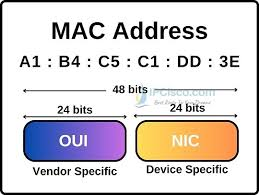
\includegraphics[width=0.5\textwidth]{pictures/mac.jpeg}
      \caption{MAC address structure \cite{MAC}}
      \label{fig:MAC}
  \end{figure}

  \subsection{\label{sec:Privacy}What are the privacy implications of a MAC address?}
  \subsection{\label{sec:Where}Where are MAC addresses used?}
    % \subsubsection{\label{subsec:Network}Network}
    \subsubsection{\label{subsec:Wi-Fi}Wi-Fi - Ethernet}
  % Dans le contexte des réseaux informatiques, les adresses MAC sont utilisées
  % pour identifier les appareils sur un réseau local.
  % Elles sont liées à l'adresse IP d'un appareil et sont utilisées pour acheminer
  % les paquets de données vers la bonne destination.
  % Le protocole ARP (Address Resolution Protocol) est utilisé pour associer une
  % adresse IP à une adresse MAC.
  % En anglais:
  In the context of computer networks, MAC addresses are used to identify devices on a local network.
  They are linked to the IP address of a device and are used to route data packets to the correct destination.
  The Address Resolution Protocol (ARP) is used to associate an IP address with a MAC address.

  \begin{figure}[H]
      \centering
      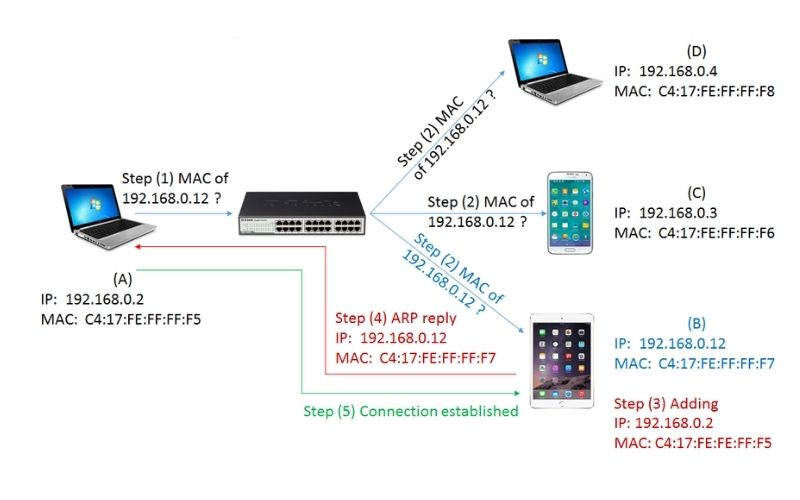
\includegraphics[width=0.5\textwidth]{pictures/arp.jpg}
      \caption{ARP protocol \cite{ARP}}
      \label{fig:ARP}
  \end{figure}
  We can see in the figure \ref{fig:ARP} that the MAC address is used to identify the device in the network.



    % ARP
    \subsubsection{\label{subsec:Bluetooth}Bluetooth}
    Bluetooth devices do not use MAC addresses in the same way as Wi-Fi devices.
    Instead, they use a 48-bit Bluetooth device address (BD\_ADDR) that is similar to a MAC address.
    BD\_ADDRs are also globally unique and could be used to track devices in the same way as MAC addresses.
    \begin{figure}[H]
        \centering
        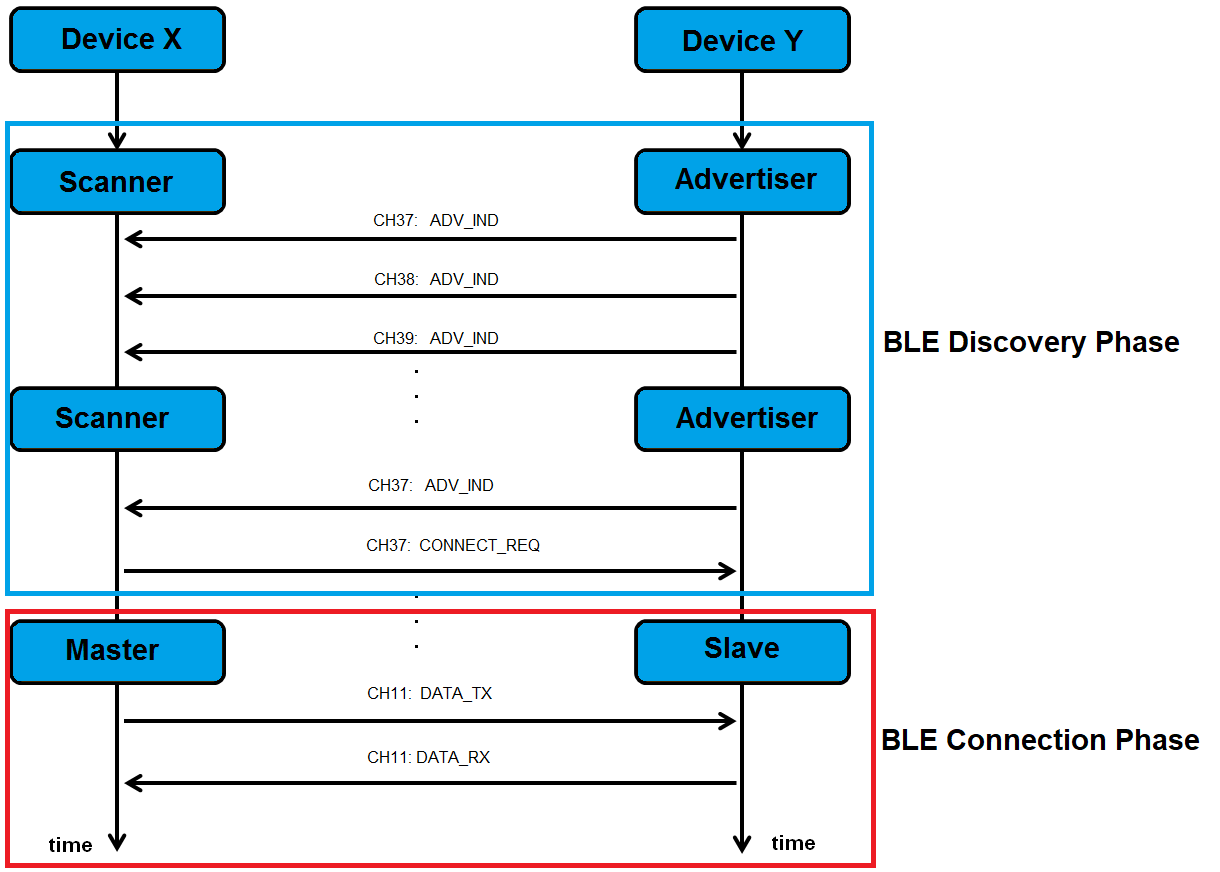
\includegraphics[width=0.5\textwidth]{pictures/Link-Layer-Roles-Change_ver1.png}
        \caption{BTLE Link Layer \cite{BLE5}}
        \label{fig:BT}
    \end{figure}
    We can see in the figure \ref{fig:BT} that even during the discovery phase, there
    is exchange in both directions, which means that the BT\_ADDR have already been 
    exchanged before even connecting to the device.


\section{\label{sec:Law}What does the law say ?}
  \subsection{\label{subsec:GDPR}GDPR}
  % \enquote{
  ``The principles of data protection should apply to any information concerning an
  identified or identifiable natural person. 
  Personal data which have undergone pseudonymisation, which could be attributed to a natural person by
  the use of additional information should be considered to be information on an identifiable natural person. To
  determine whether a natural person is identifiable, account should be taken of all the means reasonably likely to
  be used, such as singling out, either by the controller or by another person to identify the natural person directly
  or indirectly. To ascertain whether means are reasonably likely to be used to identify the natural person, account
  should be taken of all objective factors, such as the costs of and the amount of time required for identification,
  taking into consideration the available technology at the time of the processing and technological developments.
  \ul{The principles of data protection should therefore not apply to anonymous information}, namely information
  which does not relate to an identified or identifiable natural person or to personal data rendered anonymous in
  such a manner that the data subject is not or no longer identifiable. This Regulation does not therefore concern
  the processing of such anonymous information, including for statistical or research purposes.`` \cite{GDPR2016}
  % }

  \subsection{\label{subsec:ECHR}European Convention on Human Rights}
  \begin{enumerate}
    \item[34.] ``Individual applications
  The Court may receive applications from any person, non-
  governmental organisation or group of individuals claiming to be
  the victim of a violation by one of the High Contracting Parties of
  the rights set forth in the Convention or the Protocols thereto. The
  High Contracting Parties undertake not to hinder in any way the
  effective exercise of this right.``

\item[35.] ``Admissibility criteria
\end{enumerate}
  \begin{enumerate}
    \item[1.] [...]
    \item[2.] \ul{The Court shall not deal with any application submitted under Article 34 that}
    \begin{enumerate}
      \item \ul{is anonymous}; or [...]`` \cite{ECHR1950}
    \end{enumerate}
  \end{enumerate}

  \subsection{\label{subsec:Conv108}Convention 108+}
    \begin{enumerate}
      \item[18.] ``The notion of “identifiable” refers not only to the
    individual’s civil or legal identity as such, but also to
    what may allow to “individualise” or single out (and
    thus allow to treat differently) one person from others.
    This “individualisation” could be done, for instance, by
    referring to him or her specifically, or to a device or
    a combination of devices (computer, mobile phone,
    camera, gaming devices, etc.) on the basis of an iden-
    tification number, a pseudonym, biometric or genetic
    data, location data, an IP address, or other identifier.
    \ul{The use of a pseudonym or of any digital identifier/
    digital identity does not lead to anonymisation of 
  the data} as the data subject can still be identifiable
    or individualised. Pseudonymous data is thus to be
    considered as personal data and is covered by the
    provisions of the Convention. The quality of the pseud-
    onymisation techniques applied should be duly taken
    into account when assessing the appropriateness of
    safeguards implemented to mitigate the risks to data
    subjects.``

  \item[19.] ``\ul{Data is to be considered as anonymous only as
    long as it is impossible to re-identify the data subject
    or if such re-identification would require unreasonable
  time, effort or resources}, taking into consideration the
    available technology at the time of the processing
    and technological developments. Data that appears
    to be anonymous because it is not accompanied by
    any obvious identifying element may, nevertheless
    in particular cases (not requiring unreasonable time,
    effort or resources), permit the identification of an
    individual. This is the case, for example, where it is
    possible for the controller or any person to identify
    the individual through the combination of different
    types of data, such as physical, physiological, genetic,
    economic, or social data (combination of data on the
    age, sex, occupation, geolocation, family status, etc.).
    Where this is the case, the data may not be considered
    anonymous and is covered by the provisions of the
    Convention.``

  \item[20.] ``\ul{When data is made anonymous, appropriate
    means should be put in place to avoid re-identification
  of data subjects}, in particular, all technical means
    should be implemented in order to guarantee that
    the individual is not, or is no longer, identifiable. They
    should be regularly re-evaluated in light of the fast
    pace of technological development.``\cite{Conv108+}
    \end{enumerate}
    

  \subsection{\label{subsec:BEL}Belgian Law}

  Articles 101, 134, and 164 of the Belgian Act of 30 July 2018 on the protection
  of individuals with regard to the processing of personal data
  stipulate that the personal data referred to in
  \ul{Articles 99, 132, and 162 must be anonymized before they can be accessed.} 
  These articles primarily concern the processing of personal data for historical, 
  scientific, or statistical purposes.

    \begin{enumerate}
    \item[99.] ``outlines conditions under which personal data from intelligence 
    and security services can be consulted for such purposes. The consultation 
    is authorized only if it does not conflict with the service’s mandate, obligations 
    under the Act of 30 November 1998, ongoing investigations, or international relations. 
    Any request for further processing of such data for other purposes will be refused 
    unless deemed legitimate by the concerned service.``

    \item[132.] ``allows the consultation of personal data held by authorities or 
    appeal boards for historical, scientific, or statistical purposes. However, 
    it is conditional on ensuring that it does not harm any interests protected 
    under the Act of 11 December 1998, particularly regarding the confidentiality 
    and protection of personal data.``

    \item[162.] ``similarly authorizes the consultation of personal data from CUTA 
    (the Coordination Unit for Threat Analysis) for historical, scientific, or 
    statistical purposes. Again, this is contingent on ensuring no harm to CUTA’s 
    mandate, ongoing investigations, or international relations. Any requests for 
    further processing of such data for different purposes will be denied unless 
    the processing is considered legitimate and does not interfere with the 
    protected interests.``
    \end{enumerate}
  \cite{BelgianAct2018}

\section{\label{sec:Who}Who can access a MAC address?}
% More ideas in whoAndWhy.txt file 
  In fact, anyone can access a MAC address. It is transmitted in clear text over 
  the network and can be easily intercepted by anyone with the right tools. The privacy risks associated
  with MAC addresses are not limited to a specific group of people or organizations.
  However, the real issue arises when a specific location is associated with a 
  MAC address at a particular time, such as when connecting to a Wi-Fi network. 
  The problem becomes even more serious when this data is recorded, as recording 
  real-time location information can enable tracking of an individual over an 
  extended period.

  The critical question then becomes: who would have an interest in recording this data, and why? 

  \subsection{\label{subsec:ISP}Internet Service Provider}
  Internet Service Providers (ISPs) can access MAC addresses when users connect to their network.
  By definition, they have access to all the data that passes through their network, including MAC addresses.
  This data can be used for various purposes, such as network management, troubleshooting, 
  and targeted advertising. However, ISPs are subject to data protection regulations,
  and the use of MAC addresses for tracking or profiling purposes is generally prohibited.

  \subsection{\label{subsec:Audience}Audience Measurement}
  Because of the probes and probe requests, MAC addresses can be collected by anyone with a Wi-Fi-enabled device.
  This includes audience measurement companies, which collect data on the behavior of users in public spaces.
  So audience measurement companies can access MAC addresses when users walk by their Wi-Fi sensors.
  This data can be used to analyze foot traffic, measure the effectiveness of advertising campaigns,
  and provide insights to retailers and other businesses. However, the use of MAC addresses for audience measurement
  is subject to data protection regulations, and the data must be anonymized to protect the privacy of users.


\section{\label{sec:Risks}What are the risks related to MAC address?}
  \subsection{\label{subsec:Tracking}Tracking}
  % Les adresses MAC, uniques à chaque appareil, permettent une surveillance continue lorsque l'appareil interagit avec des points d'accès WiFi, des bornes Bluetooth, ou même des équipements réseau passifs. Ces interactions, qui peuvent inclure des requêtes de connexion ou de découverte, facilitent la collecte d'informations sur les déplacements des utilisateurs dans des lieux physiques comme les aéroports, les magasins, ou les rues. Par exemple, des systèmes de gestion de foule utilisent ces données pour analyser les flux de visiteurs, mais ces informations peuvent également être utilisées à des fins moins éthiques, comme la surveillance ciblée. Cela soulève des préoccupations majeures en matière de vie privée
  % En anglais:
  MAC addresses, unique to each device, allow for continuous monitoring when the 
  device interacts with Wi-Fi access points, Bluetooth beacons, or even passive network equipment.
  These interactions, which can include connection or discovery requests, facilitate 
  the collection of information about users' movements in physical locations such as airports,
  stores, or streets. For example, crowd management systems use this data to analyze visitor
  flows, but this information can also be used for less ethical purposes, such as targeted surveillance.
  This raises major privacy concerns.




  \subsection{\label{subsec:Profiling}Profiling}
  % Les données collectées via les adresses MAC peuvent être corrélées avec d'autres informations, telles que des horaires de connexion, des localisations précises, ou des modèles d'utilisation. Ces informations permettent de créer des profils détaillés des utilisateurs, révélant leurs habitudes personnelles, leurs routines quotidiennes, ou même leurs préférences en matière de consommation. Les entreprises exploitent souvent ces données pour des campagnes publicitaires ciblées, tandis que des acteurs malveillants pourraient les utiliser pour des attaques d'ingénierie sociale. Ce profilage, bien que souvent invisible pour les utilisateurs, constitue une intrusion significative dans leur vie privée
  % En anglais:
  Data collected via MAC addresses can be correlated with other information, 
  such as connection times, precise locations, or usage patterns. This information
  can be used to create detailed user profiles, revealing their personal habits, daily routines,
  or even consumption preferences. Companies often exploit this data for targeted advertising campaigns,
  while malicious actors could use it for social engineering attacks. This profiling, 
  although often invisible to users, constitutes a significant intrusion into their privacy.


  \subsection{\label{subsec:Reidentification}Re-identification}
  % Même lorsque les adresses MAC sont aléatoires (par exemple, grâce à des mécanismes d'anonymisation intégrés comme dans iOS ou Android), elles peuvent souvent être ré-identifiées en combinant différentes sources de données. Des chercheurs ont montré que des motifs d'utilisation spécifiques, tels que la durée ou la fréquence des connexions, permettent de relier une adresse MAC temporaire à son adresse originale. Cela compromet gravement les mesures d'anonymisation et expose les utilisateurs à des risques, notamment lorsque des bases de données volées ou mal sécurisées contiennent ces informations​
  % En anglais:
  Even when MAC addresses are randomized (e.g., through built-in anonymization 
  mechanisms as in iOS or Android), they can often be re-identified by combining
  different data sources. Researchers have shown that specific usage patterns,
  such as connection duration or frequency, can link a temporary MAC address to its original address.
  This seriously compromises anonymization measures and exposes users to risks,
  especially when stolen or poorly secured databases contain this information.

  \subsection{\label{subsec:Spoofing}Spoofing}
  % Le spoofing d'adresses MAC est une technique répandue, permettant à des attaquants de falsifier leur identité réseau. Cela peut être utilisé pour contourner des listes d'accès basées sur les adresses MAC (comme dans les réseaux WiFi protégés) ou pour voler l'identité d'un appareil afin d'accéder à des ressources restreintes. Ce type d'attaque est particulièrement problématique dans les environnements où des systèmes critiques reposent sur des adresses MAC pour leur fonctionnement, comme les systèmes IoT (Internet of Things). Il illustre les limites de l'utilisation des adresses MAC comme identifiants sécurisés​
  % En anglais:
  MAC address spoofing is a common technique that allows attackers to falsify their network identity.
  This can be used to bypass MAC address
  access lists (as in protected WiFi networks) or to steal a device's identity to access restricted resources.
  This type of attack is particularly problematic in environments where critical 
  systems rely on MAC addresses for their operation, such as Internet of Things (IoT) systems. 
  It illustrates the limitations of using MAC addresses as secure identifiers.



\section{\label{sec:Methods}How to anonymize a MAC address?}
  \subsection{\label{subsec:Truncation}Truncation}
  % probalilistic explanation
  % La truncation consiste à raccourcir l'adresse MAC en gardant seulement une partie de celle-ci. Par exemple, on pourrait conserver seulement les 6 premiers octets (qui correspondent généralement au fabricant), ou encore une portion aléatoire de l'adresse. Cette méthode peut permettre de garder une partie de l'information tout en minimisant le lien entre l'adresse MAC et un individu.

  %   Pourquoi cette méthode ? : Elle permet de rendre l'adresse moins identifiable, tout en gardant une certaine utilité, notamment pour les analyses statistiques où seule une partie de l'adresse est nécessaire (par exemple, l'identification du fabricant).

  %   Avantages :
  %       Simple à mettre en œuvre : La méthode est facile à implémenter et rapide.
  %       Moins de risque de ré-identification, car la portion d'adresse MAC restante ne contient pas suffisamment d'information pour être associée à une personne ou un appareil particulier.

  %   Inconvénients :
  %       Perte d'information : On peut perdre des données pertinentes si une identification plus fine de l'adresse MAC est nécessaire.
  %       Peut ne pas être suffisant pour des niveaux plus élevés d'anonymat, car la partie restante de l'adresse peut encore être utilisée pour tracer des appareils sur de longues périodes.
  % en anglais:
  Truncation involves shortening the MAC address by keeping only part of it.
  For example, you could keep only the first 6 octets (which typically correspond to the manufacturer),
  or a random portion of the address. This method can keep some of the information while minimizing 
  the link between the MAC address and an individual.

  \begin{itemize}
    \item Advantages:
      \begin{itemize}
      \item Simple to implement: The method is easy to implement and quick.
      \item Less risk of re-identification, as the remaining portion of the MAC address does not contain enough information to be associated with a particular person or device.
      \end{itemize}
    \item Disadvantages:
      \begin{itemize}
      \item Loss of information: Relevant data may be lost if a finer identification of the MAC address is needed.
      \item May not be sufficient for higher levels of anonymity, as the remaining part of the address can still 
        be used to trace devices over long periods.
      \end{itemize}
  \end{itemize}



  \subsection{\label{subsec:Hashing}Hashing}
  % multi salted hash
  %
  % Le hashing consiste à appliquer une fonction mathématique qui prend l'adresse MAC comme entrée et génère une sortie de taille fixe, appelée "haché". Ce processus est irréversible, ce qui signifie qu'il n'est pas possible de retrouver l'adresse MAC originale à partir de son haché. Une des techniques populaires pour améliorer la sécurité du hashing est l'ajout de salt.

  %   Pourquoi utiliser le salt : Le salt est une valeur aléatoire ajoutée à l'adresse MAC avant de la hasher. Cela permet de protéger contre les attaques de type rainbow table, où un attaquant aurait une pré-computation des hachages de différentes adresses MAC possibles. Le salt rend chaque hachage unique, même si deux utilisateurs ont la même adresse MAC.

  %   Utilité dans votre problématique : Le hashing avec salt est utile pour anonymiser les adresses MAC tout en permettant une certaine sécurité. Lors de la collecte de données, vous pouvez anonymiser l'adresse MAC sans risquer de déduire son origine, ce qui répond à des préoccupations légales concernant la confidentialité.

  %   Avantages :
  %       Irreversible : Une fois hachée, l'adresse MAC ne peut pas être retrouvée.
  %       Protection contre les attaques de pré-calcul (rainbow table) avec l'utilisation du salt.
  %       Facile à mettre en œuvre dans les systèmes où l'accès à l'adresse MAC originale n'est pas nécessaire après l'anonymisation.

  %   Inconvénients :
  %       Perte de l'intégrité originale : Une fois hachée, l'adresse MAC originale est complètement perdue.
  %       Si vous avez besoin de retrouver l'adresse MAC originale pour des raisons légitimes (par exemple, pour l'audit ou la réidentification dans des cas particuliers), cela peut poser un problème.

  % en anglais:
  Hashing involves applying a mathematical function that takes the MAC address as input 
  and generates a fixed-size output, called a "hash." This process is irreversible,
  meaning that it is not possible to recover the original MAC address from its hash.
  One popular technique to enhance the security of hashing is the addition of salt.

  Why use salt: Salt is a random value added to the MAC address before hashing.
  This protects against rainbow table attacks, where an attacker would have pre-computed
  hashes of different possible MAC addresses. 
  The salt makes each hash unique, even if two users have the same MAC address.

  Relevance to your problem: Hashing with salt is useful for anonymizing MAC addresses
  while providing some security. When collecting data, you can anonymize the MAC address
  without risking deducing its origin, addressing legal concerns regarding privacy.

  \begin{itemize}
    \item Advantages:
      \begin{itemize}
      \item Irreversible: Once hashed, the MAC address cannot be recovered.
      \item Protection against pre-computation attacks (rainbow table) with the use of salt.
      \item Easy to implement in systems where access to the original MAC address is not 
      needed after anonymization.

      \end{itemize}
    \item Disadvantages:
      \begin{itemize}
      \item Loss of original integrity: Once hashed, the original MAC address is completely lost.
      \item If you need to recover the original MAC address for legitimate reasons 
      (e.g., auditing or re-identification in specific cases), this can be a problem.
      \end{itemize}
  \end{itemize}



  \subsection{\label{subsec:Encryption}Encryption}
  % L'encryption consiste à chiffrer l'adresse MAC à l'aide d'un algorithme de chiffrement symétrique ou asymétrique. Dans le cas où vous avez besoin de retrouver l'adresse MAC originale à des fins légales ou administratives, l'encryption peut être utilisée, car elle permet de récupérer les données en utilisant une clé de déchiffrement.

  %   Schéma de chiffrement recommandé : DHIES : Le Diffie-Hellman Integrated Encryption Scheme (DHIES) est une méthode de chiffrement hybride qui combine l'échange de clés Diffie-Hellman et l'encryption symétrique (par exemple, AES). Ce schéma est utilisé dans des systèmes où la confidentialité des données est cruciale tout en permettant une récupération contrôlée.

  %   Pourquoi utiliser DHIES : Ce schéma offre un niveau de sécurité très élevé en utilisant une méthode d'échange de clé sécurisée (Diffie-Hellman) pour établir un canal de communication sûr, puis en utilisant un algorithme de chiffrement symétrique pour protéger les données. Il est particulièrement adapté lorsque l'accès aux données originales doit être limité et contrôlé.

  %   Avantages :
  %       Haute sécurité : Les données sont protégées de manière très robuste, avec un double niveau de sécurité.
  %       Permet de récupérer l'adresse MAC originale avec la bonne clé de déchiffrement.
  %       Idéal dans un contexte où l'anonymisation doit être réversible sous des conditions strictes.

  %   Inconvénients :
  %       Complexité : Le processus de mise en œuvre est plus complexe que les autres méthodes.
  %       Gestion des clés : La sécurité du système repose sur la gestion correcte des clés de déchiffrement, ce qui peut être un défi dans les systèmes à grande échelle.
  %       Performances : Le chiffrement et le déchiffrement peuvent introduire des frais généraux en termes de performance, particulièrement dans des systèmes à grande échelle.
  % en anglais:
  Encryption involves encrypting the MAC address using a symmetric or asymmetric encryption algorithm.
  In cases where you need to recover the original MAC address for legal or administrative purposes,
  encryption can be used, as it allows data to be recovered using a decryption key.

  Recommended encryption scheme: DHIES: The Diffie-Hellman Integrated Encryption Scheme (DHIES) 
  is a hybrid encryption method that combines Diffie-Hellman key exchange and symmetric encryption
  (e.g., AES). This scheme is used in systems where data confidentiality is crucial 
  while allowing controlled recovery.

  Why use DHIES: This scheme offers a very high level of security by using a secure key exchange method
  (Diffie-Hellman) to establish a secure communication channel, then using a symmetric encryption algorithm
  to protect the data. It is particularly suitable when access to the original data needs to be 
  limited and controlled.

  \begin{itemize}
    \item Advantages:
      \begin{itemize}
      \item High security: Data is protected very robustly, with a double layer of security.
      \item Allows recovery of the original MAC address with the correct decryption key.
      \item Ideal in a context where anonymization needs to be reversible under strict conditions.
      \end{itemize}
    \item Disadvantages:
      \begin{itemize}
      \item Complexity: The implementation process is more complex than other methods.
      \item Key management: System security relies on proper management of decryption keys, 
      which can be challenging in large-scale systems.
      \item Performance: Encryption and decryption can introduce overhead in terms of performance, 
      particularly in large-scale systems.
      \end{itemize}
  \end{itemize}


\section{\label{sec:Notable incidents}Notable incidents}
  \subsection{\label{subsec:Nordstrom}Privacy violation}
  % 2013 Nordstrom tracking customers in store 
  % https://www.forbes.com/sites/kashmirhill/2013/05/23/nordstroms-wi-fi-tracking-raises-privacy-questions/?sh=3b3b3b7b7b7b
  As part of enhancing customer experience and optimizing operations, Nordstrom has 
  implemented technology to track customer movements in its stores through their 
  Wi-Fi connections. This anonymous technology aims to analyze in-store traffic, 
  adjust staffing levels, and rethink department layouts. Since October 2012, 
  sensors in stores collect information on the time customers spend in departments, 
  without following them across sections or identifying personal details.
  Euclid has experienced rapid growth, increasing by 11,949\% in 2012. 
  The service helps retailers analyze customer flow, conversion rates, and 
  optimize workforce management based on traffic patterns. Retailers can adjust 
  staffing levels to maximize sales during peak times and reduce costs during slower periods.

  However, after testing the technology in select stores, Nordstrom announced in May 2013 
  that it would no longer use Euclid, stating that the trial had concluded and that 
  customer feedback would be incorporated into future innovations.\cite{Nordstrom2013}


  \subsection{\label{subsec:Google}Google Street View}
  % 2010 Google Street View collecting MAC addresses
  % https://www.theguardian.com/technology/2010/may/15/google-admits-storing-private-data
  Since 2007, Google Street View cars, in addition to photographing streets,
have also collected information from domestic Wi-Fi networks to improve location
services. Although this collection was accidental and involved only fragments of
data from open Wi-Fi networks, the situation raised concerns about the security
of personal data on these networks. Google admitted to collecting excerpts of personal
web activity through its Street View cars. This collection was discovered during
a data audit by Germany's data protection authority. Although Google stated it didn't
collect sensitive data, the audit revealed that it had inadvertently gathered fragments
of data from open Wi-Fi networks, though it was never used in any Google products.
Google immediately halted the collection, isolated the data, and plans to delete it
under third-party supervision. This highlights the vulnerability of data on unsecured
Wi-Fi networks.\cite{Google2007}

  \subsection{\label{subsec:London}Retail and public space tracking scandals}
  % 2013 Renew London smart bins tracking MAC addresses
  In London, a pilot project to track smartphones recorded the unique MAC addresses
of over half a million phones through a network of recycling bins. Located at 12 spots,
these bins captured the MAC addresses of phones with Wi-Fi on, as well as data on the
movement, direction, and speed of the devices. The project, run by Renew London, demonstrates
the potential for targeted advertising by analyzing users' past behaviors, such as their
workplaces, places of interest, and habits. During tests in May and June, over four million
events were captured, involving more than 530,000 unique devices. While the data is collected
anonymously, Renew emphasized that the devices are not individually tracked and the data
is aggregated. However, it remains unclear whether this collection violates the Data Protection
Act, as MAC addresses may be considered personal data.\cite{RenewLondon2013}


  \subsection{\label{subsec:DataLeaks}Data Leaks and Security Breaches Involving MAC Data}
  % 2017 Equifax data breach
  % 2018 Exactis data breach
  % 2015 VTech data breach
  \subsection{\label{subsec: Attacks}Attacks Exploiting MAC Addresses}
  % Man-in-the-middle attacks in airports and cybercafes
  \subsection{\label{subsec:WhatsApp}WhatsApp Security Vulnerability}

% En 2012, une faille de sécurité a été découverte dans WhatsApp, permettant à un 
% attaquant d'usurper l'identité d'un utilisateur si l'adresse MAC de son appareil 
% pouvait être obtenue. À cette époque, WhatsApp n’utilisait pas de chiffrement de 
% bout en bout et s’appuyait sur l’adresse MAC de l’appareil pour authentifier les 
% utilisateurs. 

% En exploitant cette faille, un attaquant pouvait :
%     Se connecter au compte WhatsApp de la victime depuis un autre appareil.
%     Lire et envoyer des messages comme si c’était la victime.

% Exploitation de la faille :
% Les attaquants pouvaient obtenir l'adresse MAC via différents moyens, notamment par 
% des attaques sur des réseaux Wi-Fi publics ou via des applications malveillantes 
% capables de lire l'adresse MAC d'un appareil. Ensuite, ils pouvaient utiliser des 
% outils spécifiques pour se connecter à WhatsApp en se faisant passer pour la victime.

% Conséquences et correction :
% Ce problème a mis en lumière les risques d'utiliser des identifiants statiques comme 
% les adresses MAC pour authentifier les utilisateurs. WhatsApp a finalement renforcé 
% ses mesures de sécurité, notamment en adoptant le chiffrement de bout en bout, et a 
% cessé d’utiliser l’adresse MAC pour l’authentification.

% Ce cas montre l'importance de ne pas se fier aux adresses MAC pour authentifier les 
% utilisateurs, en raison de la facilité avec laquelle elles peuvent être usurpées.
% en anglais:
In 2012, a security vulnerability was discovered in WhatsApp that allowed an attacker 
to impersonate a user if the MAC address of their device could be obtained. At that time,
WhatsApp did not use end-to-end encryption and relied on the device's MAC address to authenticate users.
By exploiting this vulnerability, an attacker could:
    \begin{itemize}
    \item Log into the victim's WhatsApp account from another device.
    \item Read and send messages as if they were the victim.
    \end{itemize}

Exploitation of the vulnerability:
Attackers could obtain the MAC address through various means, including attacks on public Wi-Fi networks
or through malicious applications capable of reading a device's MAC address. They could then use specific tools
to log into WhatsApp while posing as the victim.

Consequences and fix:
This issue highlighted the risks of using static identifiers like MAC addresses to authenticate users.
WhatsApp eventually strengthened its security measures, including adopting end-to-end encryption, 
and stopped using the MAC address for authentication. This case illustrates the importance 
of not relying on MAC addresses to authenticate users due to how easily they can be spoofed.






\section{\label{sec:Conclusion}Conclusion}
In conclusion, MAC addresses, while essential for network communication, present 
significant privacy risks when not properly anonymized or protected. The ability 
to track devices based on their MAC address has raised concerns about surveillance 
and unauthorized data collection, especially when these addresses are linked to 
individuals or their activities. The legal landscape, particularly the GDPR and 
other international standards, plays a critical role in regulating the use of 
personal data, including MAC addresses, and emphasizes the need for robust privacy 
protections. Anonymization techniques, such as pseudonymization and encryption, 
are essential to mitigate these risks, ensuring that MAC addresses can be used 
without compromising user privacy. As the IoT ecosystem continues to grow, the 
importance of developing effective anonymization strategies will be pivotal in 
safeguarding personal data and upholding privacy rights in embedded systems and 
beyond.
\subsection{\label{sec:Why}Why should we anonymize a MAC address?}


\bibliographystyle{unsrt}
\bibliography{bibliography}

\end{document}
